\documentclass[a4paper,spanish]{article}
\usepackage[activeacute]{babel}
\usepackage[utf8]{inputenc}
\usepackage{listings}
\usepackage{graphicx}
\usepackage{epsfig}
\usepackage{riesgos}
\usepackage[font=small,labelfont=bf]{caption}
\hoffset=-2.5cm
\textwidth=17cm
\parskip=1ex



%opening
\title{Ingeniería de Software II\\ \textbf{Sistema ``Twitteando para Ahorrar''}}
\author{\textbf{Grupo 6}\\ 1º Cuatrimestre 2013} 
\date{}


\begin{document}

\maketitle
\vspace{10cm}
\begin{center}

\begin{tabular}{|c|c|c|}
\hline
\hline
\textbf{LU}&\textbf{Nombre}&\textbf{email}\\
\hline
667/06&Daniel Foguelman &dfoguelman@dc.uba.ar\\
\hline
767/03&Hernán Modrow&hmodrow@gmail.com\\
\hline
511/00&Leonardo Tilli&leotilli@gmail.com\\
\hline
\hline
\end{tabular}
\end{center}
\newpage

\section{Parte I}

 En este informe presentamos la planificación para el proyecto TPA para las etapas subsiguientes a lo creado en la entrega anterior. En este proceso, integraremos el Core de Twiteando para Ahorrar con múltiples servicios (Redes sociales, detección de fraude, etc), tendremos requerimientos funcionales y no-funcionales de media y gran complejidad. Esto Nos mueve del paradigma SCRUM por uno más tradicional, RUP, haciendo preponderancia en la planificación y análisis de requerimientos antes que en la adaptabilidad al cambio y visibilidad del proyecto. \\

 El plan desarrollado para esta nueva etapa sigue el modelo RUP, y se documenta a continuaci\'n. Primero se describir\'an los casos de uso identificados. En base a esto se detallan las distintas iteraciones que se planificaron y de qu\'e consta cada una. En la \'ultima secci\'on se encuentra el an\'alisis de los riesgos m\'as importantes que se detectaron.


\section*{Lista de Casos de Uso}

\section*{Riesgos}

%Template
%\begin{riesgo}{SITUACION}{CONSECUENCIA}
%    \contexto{Texto de contexto}
%    \probabilidad{Baja-Media-Alta}
%    \impacto{Cr\'itico-Medio-Bajo}
%    \exposicion{Alta-Media-Baja}
%    \mitigacion{Texto mitigacion}
%    \contingencia{Texto contingencia}
%\end{riesgo}

\begin{riesgo}{el/los cluster/s armados pueden no tener suficiente poder de computo}{los tiempos de respuesta y el conjunto de datos analizados no sean los esperados.}
    \contexto{Se espera manejar grandes vol\'umenes datos y de peticiones por lo tanto necesita alto poder de procesamiento y una gran cantidad de espacio para almacenarse.}
    \probabilidad{Media}
    \impacto{Alto}
    \exposicion{Alta}
    \mitigacion{Diseñar arquitectura que escale horizontalmente y sea f\'acil agregar capacidad de procesamiento y de datos.}
    \contingencia{Disminuir la cantidad de informaci\'on que se puede recibir y enviar TPA a los usuarios. Analizar la distribuci\'on del sistema en nodos que abarquen las consultas de determinadas regiones.}
\end{riesgo}

\begin{riesgo}{la arquitectura se define con computadores de bajo costo}{se ca\'iga la base de datos con la informaci\'on de las ofertas}
    \contexto{La ca\'ida de la infraestructura de repositorios de ofertas generar\'ia una caida del servicio completo.}
    \probabilidad{Baja}
    \impacto{Alta}
    \exposicion{Media}
    \mitigacion{Informaci\'on guardada con chequeos de integridad que permitan una f\'acil recuperaci\'on (RAID). Redundancia de la base de datos con informaci\'on de la ofertas.}
    \contingencia{Recuperar la informaci\'on utilizando chequeo de integridad de datos. Levantar sistemas de base de datos de backup.}
\end{riesgo}

\begin{riesgo}{el sistema se espera sea usado masivamente}{se genere mucha carga en el uso del sistema que produzca lentitud de respuesta}
    \contexto{Dado que el sistema TPA tendr\'a impacto a nivel nacional y regional, es esperable una gran carga de consultas.}
    \probabilidad{Alta}
    \impacto{Alta}
    \exposicion{Alta}
    \mitigacion{Generar una arquitectura que permita la alta disponibilidad del servicio utilizando \textbf{cach\'es} distribuidos para minimizar la carga en cada servidor. Armar casos de tests espec\'ificos para detectar problemas de disponibilidad en el sistema.}
    \contingencia{Levantar clusters adicionales, en caso de no ser posible evaluar la contrataci\'on de clusters externos.}
\end{riesgo}

\begin{riesgo}{se quiere que el sistema sea usado por la mayor cantidad de gente y en la mayor cantidad de plataformas}{no sea homogeneo entre las distintas plataformas y f\'acil de usar para todos los usuarios}
    \contexto{La aplicaci\'on TPA deber\'a tener alcance nacional y ser inclusiva para todos y todas. Las personas de edad avanzada o con capacidades especiales deber\'an poder utilizar las interfaces de usuario de manera intuitiva.}
    \probabilidad{Bajo}
    \impacto{Bajo}
    \exposicion{Baja}
    \mitigacion{Buscar especialistas en usabilidad para generar interfaces aptas.}
    \contingencia{No hacer nada, el porcentaje de estos usuarios es menor en comparaci\'on a los usuarios activos.}
\end{riesgo}

\begin{riesgo}{los servicios del sistema se proveer\'an a trav\'es de Internet}{recibir un ataque de Denegaci\'on de Servicio (DoS y DDoS) no siendo posible brindar los servicios}
    \contexto{Existen grupos de activistas que con distintas motivaciones atacan sitios mediante ataques de denegaci\'on de servicio para hacer llegar su mensaje. Estos ataques son faciles de generar y ejecutables en todo tipo de computadoras, incluso celulares o tablets, por lo que pueden ser facilmente escables por un grupo coordinado.}
    \probabilidad{Media}
    \impacto{Alta}
    \exposicion{Alta}
    \mitigacion{Generar una aplicaci\'on distribuida con buena distribuci\'on de carga para poder soportar alta carga de datos. Organizar periodicamente simulaciones de este tipo de ataques para probar el sistema. }
    \contingencia{Minimizar el tiempo de reinicializaci\'on de los servicios de TPA. Analizar la distribuci\'on del sistema en nodos que abarquen las consultas de determinadas regiones. Evaluar la contrataci\'on de sistema contra este tipo de ataques.}
\end{riesgo}

\begin{riesgo}{se almacena informaci\'on de los usuarios en sistema}{esa informaci\'on sea robada}
    \contexto{Dada la exposici\'on de los usuarios as\'i como otra informaci\'on que se requiera que sea relevante al sistema, ej: configuraci\'on de confianza, h\'abitos de utilizaci\'on, dicha informaci\'on es suceptible de ser comercializada.}
    \probabilidad{Alta}
    \impacto{Medio}
    \exposicion{Alta}
    \mitigacion{Anonimizar la informaci\'on de los usuarios utilizada internamente. Aislar los datos sensibles de los usuarios de otros partes del sistema, encriptar, restringir y auditar su utilizaci\'on. Realizar simulaciones de ataques para encontrar vulnerabilidades.}
    \contingencia{Cerrar las consultas de informaci\'on y dejar solo accesible las consultas de ofertas generales.}
\end{riesgo}

\begin{riesgo}{el sistema depende en gran parte de la informaci\'on provista por lo usuarios}{haya un alto porcentaje de ofertas dudosas}
    \contexto{Dado que el proyecto es esponsoreado por el gobierno nacional, es posible que un n\'umero importante de ofertas dudosas sean generadas que buscan manipular el sistema en pos de un beneficio personal.}
    \probabilidad{Bajo}
    \impacto{Medio}
    \exposicion{Media}
    \mitigacion{Informar a los usuarios de los beneficios de usar el sistema correctamente. Buscar la adopci\'on temprana del sistema por parte de los usuarios para que estos generen un alto n\'umero de datos. Utilizar los servicios de SpamBuster para el filtrado de ofertas dudosas mientras se genera un m\'odulo proprio. Invalidaci\'on de ofertas manualmente por usuarios administrativos/configuraci\'on.}
    \contingencia{Generar listas de productos oficialmente verificados por agentes de TPA.}
\end{riesgo}

\begin{riesgo}{dado el contexto inflacionario y de polarizaci\'on pol\'itica}{informaci\'on no sea confiada por los usuarios}
    \contexto{La poca credibilidad en los \'indices inflacionarios podr\'ia inducir a la falta de confianza de los usuarios a los resultados de b\'usqueda.}
    \probabilidad{Baja}
    \impacto{Bajo}
    \exposicion{Baja}
    \mitigacion{Generaremos reportes de confianza para entender las necesidades de los usuarios y mejorar la confiabilidad de las ofertas sugeridas.}
    \contingencia{Evaluar la realizaci\'on de una campaña publicitaria para generar confianza en los usuarios. Evaluar la posibilidad de la captura de ofertas mediante fotos.}
\end{riesgo}

\begin{riesgo}{el sistema depende en gran parte de la informaci\'on provista por lo usuarios}{haya un gran n\'umero de usuarios no confiables}
    \contexto{Dado que el proyecto es esponsoreado por el gobierno nacional, es posible que se registren usuarios que hagan busquen el fracaso del sistema, ej: disminuyendo la confiabilidad de las ofertas.}
    \probabilidad{Bajo}
    \impacto{Medio}
    \exposicion{Baja}
    \mitigacion{Generar estrategias de validaci\'on de usuarios para minimizar la falsificaci\'on de identidad. Evaluar la generaci\'on programas de fidelizaci\'on fin de que los usuarios quieran registrarse utilizando informaci\'on fidedigna y participar activamente generando informaci\'on confiable.}
    \contingencia{Los usuarios deber\'an verificarse personalmente para poder utilizar el sistema.}
\end{riesgo}

\begin{riesgo}{el presupuesto es acotado y se espera que el sistema genere ingresos propios a fin de mantenerse}{los fondos obtenidos de los servicios pagos ofrecidos sean insuficientes y el proyecto fracase}
    \contexto{El proyecto depende de fondo.}
    \probabilidad{Baja}
    \impacto{Alto}
    \exposicion{Media}
    \mitigacion{Venta de servicios para sugerir ofertas de comerciantes. Venta de informaci\'on est\'adistica del sistema.}
    \contingencia{Agregar ventea publicadad al sistema. Solicitar fondos adicionales al estado nacional. Buscar fuentes de financiaci\'on adicionales.}
\end{riesgo}

\begin{riesgo}{es necesario obtener informaci\'on de ofertas distintos sistemas/p\'aginas web mediante webcrawling}{no se descubran correctamente las ofertas de los mismos}
    \contexto{La programci\'on de analizadores de leguaje natural es una tarea compleja que requiere un alto nivel de conocmiento para implementarse correctamente.}
    \probabilidad{Media}
    \impacto{Medio}
    \exposicion{Media}
    \mitigacion{Alguno de los miembros del equipo asistar\'a a una capacitaci\'on sobre el tema, para que luego realice capacitaci\'on interna. Implementaremos estrat\'egias de entrenamiento de la plataforma y generaremos m\'ultiples casos de test para verificar la identificaci\'on de ofertas. Tambi\'en utilizaremos una estrategia de supervisi\'on de la identificaci\'on de ofertas por un operario manual a fin de mejorar la detecci\'on.}
    \contingencia{Contrataremos personal que identifique las ofertas que no se est\'an encontrando para poder generar nuevas estrategias de detecci\'on.}
\end{riesgo}

\begin{riesgo}{es necesario almacenar la informaci\'on de las ofertas en un base de datos no relacional (NOSQL) y el equipo tiene poca experiencia}{de que el proyecto se atrase o de que fracase debido al mal armado del modelo de datos}
\contexto{Se solitica la utilizaci\'on de una base de datos no relacional a fin guardar la informaci\'on de las ofertas.}
\probabilidad{Alta}
\impacto{Alto}
\exposicion{Alta}
\mitigacion{Alguno de los miembros del equipo asistar\'a a una capacitaci\'on sobre el tema, para que luego realice capacitaci\'on interna.}
\contingencia{Contratar a un especialista en el tema para que participe del proyecto. Alternativamente tercerizar esa parte del proyecto.}
\end{riesgo}

\begin{riesgo}{se utilizar\'an m\'aquina es necesario armar uno (o varios) clusters y que los miembros delequipo no tienen experiencia en esto}{de que el proyecto se atrase o de que fracase en cuanto al nivel de procesamiento de datos que realiza}
\contexto{Se dispone de PCs comunes para el deploy del sistema. Dado que se requiere un alto nivel de procesamiento es que se deber\'an armar clusters con las PCs a fin de generar mayor poder de computo.}
\probabilidad{Alta}
\impacto{Alto}
\exposicion{Alta}
\mitigacion{Alguno de los miembros del equipo asistar\'a a una capacitaci\'on sobre el tema, para que luego realice capacitaci\'on interna. Destrabar la importaci\'on de los servidores dedicados.}
\contingencia{Contratar a un especialista en el tema para que participe del proyecto. Evaluar la contrataci\'on de un servicio externo de procesamiento de datos.}
\end{riesgo}

\begin{riesgo}{los fondos destinados al contrato de Spam-Bust son acotados}{haya perdida de funcionalidad control de spam}
    \contexto{Dado la partida presupuestaria a destinada al pago de acotado e incluso podr\'ia no materializarse.}
    \probabilidad{Baja}
    \impacto{Alto}
    \exposicion{Medio}
    \mitigacion{Gestionar adecuadamente los requerimientos de an\'alisis de spam para que dichos CU no se retrasen. Contratar el servicio con la posibilidad de poder diferir/postergar los pagos.}
    \contingencia{Que el equipo de desarrollo se aboque al desarrollo de la funcionalidad. Evaluar la tercerizaci\'on del desarrollo}
\end{riesgo}

\begin{riesgo}{equipo de trabajo es reducido}{un miembro de equipo renuncie y el proyecto se atrase}
    \contexto{El equipo de trabajo es pequeño (3 personas). Los miembros de equipo est\'an entusiasmados por los desaf\'ios que impone el proyecto}
    \probabilidad{Baja}
    \impacto{Alto}
    \exposicion{Medio}
    \mitigacion{Reservar fondos para una bonificaci\'on de entrega del proyecto a tiempo. Incorporar nuevos desarrolladores como backups.}
    \contingencia{Negociar replanificaci\'on del proyecto con el cliente. Conseguir reemplazo.}
\end{riesgo}


%% Reemplazado por las anteriores
%% \begin{riesgo}{la complejidad de desarrollo del proyecto es alta se precisa personal altamente calificado}{se generar\'a un producto de baja calidad}
%    % \contexto{La complejidad, dada por los sistemas de asignaci\'on de confiabilidad, la gran interacci\'on con sistemas heterogeneos, la necesidad de alta disponibilidad, etc. hace que el personal t\'ecnico que desarrollar\'a la plataforma necesite estar altamente calificado.}
%    % \probabilidad{Alta}
%    % \impacto{Cr\'itico}
%    % \exposicion{Alta}
%    % \mitigacion{Contratar personal altamente calificado y armar workshops para compartir el conocimiento de las tecnolog\'ias utilizadas en el proyecto hacia los menos calificados. Haciendo que todos los t\'ecnicos involucrados mantengan la calidad del producto.}
%    % \contingencia{Contratar un servicio de consultor\'ia de software que permita resolver los conflictos t\'encnicos que pudieran darse.}
%% \end{riesgo}
%
%\subsection*{Reveer}
%
%Estos riesgos no se leen como \textit{DADO QUE condicion EXISTE EL RIESGO QUE evento}.
%O no quedan claras las mitigaciones y/o contigencias.
%
%\begin{riesgo}{surja un retraso en la implementaci\'on de reporte de ofertas dudosas}{se falte a la necesidades del sector Defensa al Consumidor}
%    \contexto{La gente asociada al sector Defensa al Consumidor precisa este reporte para poder tomar las deciciones adecuadas, sin este el proyecto carece del aval institucional que prov\'e DC.}
%    \probabilidad{Baja}
%    \impacto{Medio}
%    \exposicion{Baja}
%    \mitigacion{Priorizar estos casos de uso para garantizar la implementaci\'on de estos.}
%    \contingencia{Proveer feedback inmediato al sector.}
%\end{riesgo}

\subsection*{Priorizaci\'on de Riesgos}

\begin{center}
    \begin{tabular}{| l | l | l |}
    \hline
	Prioridad & Riesgo & Exposici\'on \\ \hline
	1 & R1 & Alta \\ \hline
	2 &	R3 & Alta \\ \hline
	3 &	R12 & Alta \\ \hline
	4 &	R13	& Alta \\ \hline
	5 &	R5 & Alta \\ \hline
	6 &	R6 & Alta \\ \hline
	7 &	R2 & Media \\ \hline
	8 &	R10 & Media \\ \hline
	10 & R14 & Media \\ \hline
	11 &  R15 & Media \\ \hline
	9 &	R11 & Media \\ \hline
	11 & R4 & Baja \\ \hline
	12 & R7 & Baja \\ \hline
	13 & R8 & Baja \\ \hline
	14 & R9 & Baja \\ \hline
    \end{tabular}
\end{center}
\section*{Plan de Proyecto}

Considerando las posturas de los stakeholders con los que se tuvo contacto, se decidi\'o dar prioridad a la usabilidad, rendimiento, e integrabilidad y extensibilidad. Para esta segunda parte se cuenta con una dedicaci\'on \textit{full-time} de los tres integrantes del equipo.

\subsubsection{Iteraci\'on 1 - Elaboraci\'on (2 semanas / 240 horas)}	
	
	\begin{itemize}
		  \item Definici\'on de arquitectura
		  \item CU-01: Autentic\'andose al sistema
		  \item CU-02: Cargando oferta a trav\'es de la Web-API
		  \item CU-03: Consultando oferta a trav\'es de API-Internet
		  \item CU-04: Consultando oferta a trav\'es de p\'agina web TPA
		  \item CU-05: Enviando sugerencia sobre el sistema
	\end{itemize}

\textbf{Detalle de la iteraci\'on}

	Los casos de uso incluidos en esta primera iteraci\'on conforman un subconjunto m\'inimo que nos permite tener un recorrido completo de la aplicaci\'on. Esto \'ultimo implica tambi\'en que varios de \'estos tiene un alto impacto en la arquitectura, teniendo que tomar decisiones al respecto de la autenticaci\'on, implementaci\'on del servicio Web-API, integraci\'on del sitio Web-TPA con el servicio API, modelo de persistencia de entidades y resoluci\'on de b\'usquedas.
	
	La decisi\'on de generar un recorrido completo tambi\'en tiene en cuenta los riesgos relevados, dado que los riesgos de mayor exposici\'on est\'an relacionado con cuestiones de performance y arquitectura. Esto junto con la b\'usqueda de que haya una  adopci\'on temprana del sistema por parte de los usuarios, permitir\'a evaluar tempranamente el funcionamiento del sistema para corregir en una fase temprana cualquier inconveniente de arquitectura que pudiera surgir y no hubiese sido relevado.
	
	Desde el punto de la usabilidad, incluimos el env\'io de sugerencia para tener un feedback temprano del usuario. Desde el punto de vista del rendimiento, apuntamos a utilizar una interfaz simple, que minimice el intercambio de datos por consulta. Por \'ultimo, desde el punto de vista de la integrabilidad y extensibilidad, decidimos implementar todos las funcionalidades en el servicio Web-API, reutiliz\'andolo desde el sitio Web-TPA.
	
\subsubsection{Iteraci\'on 2 - Elaboraci\'on (2 semanas / 240 horas)}
	
	\begin{itemize}
	  \item CU-06: Configurando oferta sugerida (24hs)
	  \item CU-07: Buscando informaci\'on de oferta sugerida (32hs)
	  \item CU-08: Generando reporte de ofertas dudosas con Spam-Buster (64hs)
	  \item CU-21: Configurando sistema de ofertas (56hs)
	  \item CU-10: Cargando/Consultando oferta por P\'agina Web/Red Social [Twitter] (64hs)
	\end{itemize}

\subsubsection{Iteraci\'on 3 - Elaboraci\'on (2 semanas / 240 horas)}
	
	\begin{itemize}
		\item CU-10: Cargando/Consultando oferta por P\'agina Web/Red Social [cont.] (64hs)
		\item CU-09: Invalidando oferta (40hs)
		\item CU-11: Generando reporte de ofertas dudosas con M\'odulo Propio (64hs)
		\item CU-12: Registrar informacion de uso del sistema (24)
		\item CU-13: Asignando confiabilidad a oferta (48)
	\end{itemize}

\subsubsection{Iteraci\'on 4 - Construcci\'on (4 semanas / 480 horas)}
	
	Las siguientes tareas se desarrollan para finalizar con el deplyment del sistema
	
	\begin{itemize}
	  	  \item CU-14: Asignando confiabilidad a usuario (40)
		  \item CU-10: Cargando/Consultando oferta por P\'agina Web/Red Social [cont.] (40hs)
		  \item CU-15: Comparando SpamBuster con M\'odulo de ofertas dudosas (160hs)
		  \item CU-16: Configurando sistema de confianza personal (136hs)
		  \item CU-17: Mostrando mapa oferta (104hs)
	\end{itemize}

\subsubsection{Iteraci\'on 5 - Transici\'on (2 semanas / 240 horas)}
	
	\begin{itemize}
		  \item CU-10: Cargando/Consultando oferta por P\'agina Web/Red Social [cont.] (60hs)
		  \item CU-18: Analizando web en busca de ofertas (60hs)
		  \item CU-18: Cargando/Consultando oferta por SMS (64hs)
		  \item CU-20: Consultando informaci\'on estad\'istica del sistema (56 hs)
	\end{itemize}

\subsection*{Gantt de la Primera Iteraci\'on}
\begin{figure}[hbtp]
\centering
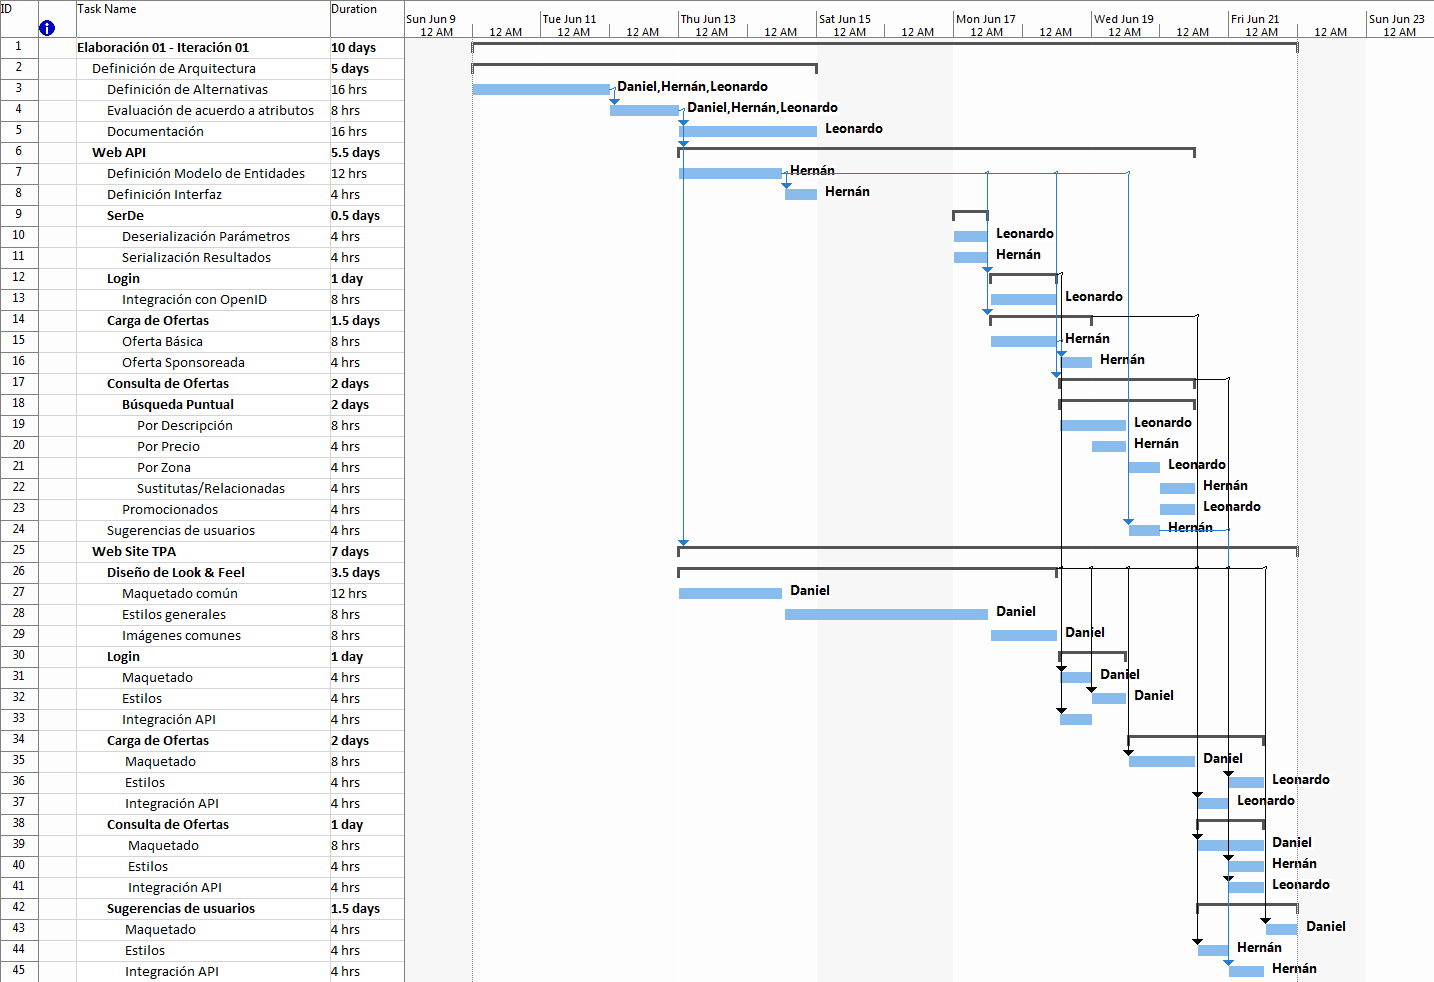
\includegraphics[height=0.75\textheight,angle=90]{TP2Planificacion}
\caption{Diagrama de Gantt de tareas de la primera iteraci\'on, con divisi\'on de tareas y asignaci\'on de recursos}
\label{fig:gantt}
\end{figure}



\end{document}
